    


\documentclass{article}
\usepackage[T1]{fontenc} % Fontes T1
\usepackage[utf8]{inputenc} % Input UTF8
\usepackage{tikz}
\usetikzlibrary{fit, shapes.geometric}
\usepackage{adjustbox}
\usepackage{multirow}
\usepackage{booktabs}
\usepackage{arydshln}
\usepackage{geometry}
\usepackage{caption}
\usepackage{float}
\usepackage{titlesec}
\usepackage{array}


\usepackage{hyperref}
\usepackage{enumerate}

\usepackage{hyperref} % Para links clicáveis
\usepackage{url}      % Para formatação de URLs (opcional)
\usepackage{xurl}     % Permite quebra de links longos automaticamente





\geometry{
  a4paper,
  hmargin=3cm,
  top=2cm,
  bottom=2cm,
}



\usepackage{csquotes}
\usepackage[portuguese]{babel} %Usar língua portuguesa
\usepackage{blindtext} % Gerar texto automaticamente
\usepackage[printonlyused]{acronym}
\usepackage{hyperref} % para autoref
\usepackage{graphicx}
\usepackage{indentfirst}
\usepackage[section]{placeins}
\usepackage{changepage}
\usepackage{adjustbox}
\usepackage{pgfplots}
\usepackage{subcaption}
\renewcommand{\baselinestretch}{1.5}

%%
% Definições
%

%
%%%%%% CAPA %%%%%%
%
\begin{document}


\def\titulo{Relatório do Projeto em Engenharia de Computadores e Informática (M2)}

\def\subtitulo{Sistema de Difusão de Áudio Digital Multi-Canal}
\def\data{DATA}
\def\autores{David Pelicano \\ Henrique Ferreira \\ Martina Duque \\ Pedro Melo \\ Sofia Marrafa \\ Tomás Oliveira }

\def\tutores{Daniel Albuquerque e Guilherme Campos}

\def\autorescontactos{(113391) davidpoetapelicano@ua.pt,\\  (113600) ferreira.manuel.henrique04@ua.pt,\\ (113261) martina.duque18@ua.pt \\ (114208) pedro.m.melo@ua.pt\\ (114591) sofiamarrafa@ua.pt\\ (113939) tomas.esteves.oliveira@ua.pt}

\def\departamento{Dept. de Eletrónica, Telecomunicações e Informática}
\def\empresa{Universidade de Aveiro}
\def\logotipo{ua.pdf}

%
%%%%%% CAPA %%%%%%
%
\begin{titlepage}

\begin{center}
%
\vspace*{40mm}
%
{\Huge \titulo}\\ 

%

\vspace{10mm}
{\Large \subtitulo}\\ 
%
\vspace{4mm}
{\Large Grupo 12}\\ 
%
\vspace{10mm}
{\Large \empresa}\\
%
\vspace{15mm}
%
{\large \autores}\\ 
%
\vspace{15mm}
{\large Supervisores: Daniel Albuquerque e Guilherme Campos} \\
\vspace{20mm}
%
\begin{figure}[h]
\center

\includegraphics{ua.pdf}
\end{figure}
%
\vspace{25mm}
\end{center}
%
\begin{flushright}

\end{flushright}
\end{titlepage}

%%  Página de Título %%
%% Página de Título
\begin{titlepage}
\begin{center}
    % Título
    \vspace*{3cm} % Ajuste este valor para baixar o título
    {\Huge\textbf{\titulo}}\\[1cm] % 1 cm de espaço abaixo do título
    
    % Subtítulo
    {\Large \subtitulo}\\[0.5cm]
    {\empresa}\\[2cm] % 2 cm de espaço abaixo da instituição
    
    % Autores
    {\large \autores}\\[1cm]
    
    % Contatos
    {\small \autorescontactos}\\[2cm]
    
    % Data
    \date{\today}
    \today
\end{center}
\end{titlepage}

%% Índice
\clearpage
\setcounter{page}{1}
\tableofcontents

\clearpage
%%%%%%%%%%%%%%%%%%%%%%%%%%%%%%%

\hspace{5cm}


\section*{Resumo}

Este projeto centra-se no desenvolvimento de um sistema de difusão de áudio digital multi-canal sem fios, concebido para proporcionar uma maior versatilidade e fidelidade sonora em diferentes ambientes. Através da utilização de tecnologias wireless, o sistema será composto por uma unidade de controlo central, responsável por gerir a distribuição eficiente de múltiplos canais de áudio para diversas colunas ativas equipadas com recetores integrados.


Esta arquitetura permitirá a criação de uma rede de áudio sincronizada, por forma a garantir uma reprodução com qualidade e a possibilidade de uma gestão remota, com personalização em tempo real das saídas de áudio. Assim, cada zona poderá ser configurada de forma independente, adaptando-se às necessidades específicas do espaço.


O desenvolvimento deste projeto abrange diversas etapas, começando pela análise e integração de tecnologias de transmissão e receção de áudio já existentes. Segue-se o design e implementação do hardware e software necessários para a unidade de controlo e os recetores, assegurando a compatibilidade e eficiência do sistema. Por fim, será realizada uma fase de testes para os diferentes cenários, de modo a garantir o desempenho e fiabilidade da solução final.




\newpage

\section{Introdução}

\vspace{1cm}


\subsection{Contexto}

\vspace{0.1cm}

Hoje em dia, o áudio desempenha um papel fundamental no nosso quotidiano, presente numa ampla variedade de contextos, desde ambientes domésticos e automóveis até espaços comerciais e institucionais. A evolução das tecnologias da transmissão sonora, como Bluetooth, Wi-Fi bem como  protocolos dedicados ao streaming de áudio, tornou o acesso a conteúdos sonoros mais prático e personalizável. Contudo, parte das soluções disponíveis centra-se no controlo do áudio no utilizador final, o que acaba por limitar uma possível gestão centralizada e consequentemente isso dificulta a coordenação eficiente em espaços partilhados.

Assim sendo, este projeto propõe então uma abordagem inovadora para a difusão de áudio digital sem fios, focando-se na distribuição inteligente e centralizada de conteúdos sonoros. O principal objetivo consistirá em desenvolver um sistema que permita a transmissão de áudio para múltiplos recetores, podendo este ajustar dinamicamente os canais de reprodução e que irá permitir garantir uma experiência auditiva consistente e adaptável às necessidades específicas de cada ambiente.

Posto isto, a proposta deste projeto promete um sistema versátil o que o torna adequado para diversos cenários, desde pequenos estabelecimentos comerciais e escritórios até infraestruturas de grande escala, como centros comerciais, hotéis, aeroportos e espaços de eventos. A implementação de um modelo centralizado não só otimiza a gestão dos conteúdos transmitidos bem como irá  facilitar a configuração e adaptação a diferentes requisitos acústicos.

Com este projeto, pretende-se explorar soluções eficientes para a transmissão de áudio sem fios, avaliando alguns fatores como latência, sincronização e qualidade sonora, de forma a garantir um bom desempenho e uma experiência auditiva adquada.

O sistema proposto iŕa basear-se em uma unidade de controlo central, responsável pela gestão e distribuição de múltiplos canais de áudio em diferentes zonas, adaptando-se dinamicamente ao ambiente e à finalidade de cada espaço. Esta abordagem permite a criação de uma rede de áudio sincronizada, onde os recetores, integrados nas colunas, garantem uma reprodução personalizada para cada área de transmissão.


A coordenação remota do áudio através do sistema central de difusão possibilita uma experiência auditiva ajustável às necessidades específicas de cada espaço, garantindo uma instalação mais simplificada devido à utilização de tecnologias sem fios. A eliminação de cablagem extensa não só reduz custos e complexidade logística, como também aumenta a flexibilidade na disposição e configuração do sistema.


O desenvolvimento deste projeto será estruturado em várias fases, abrangendo a seleção das tecnologias mais adequadas para a transmissão e receção de áudio dados os espaços para os quais as transmissões vão ser realizadas, o desenvolvimento do hardware e firmware necessários, e a realização de testes para avaliar fatores como qualidade de som e latência do sistema em diferentes cenários de utilização. O objetivo final é criar uma solução fiável e de fácil implementação, capaz de atender às exigências de espaços de diferentes dimensões e finalidades, desde pequenos estabelecimentos comerciais até grandes infraestruturas como centros comerciais, hotéis e espaços de conferências.


Este projeto será conduzido sob a orientação de professores do Departamento de Eletrónica, Telecomunicações e Informática, em colaboração com o Instituto de Telecomunicações, proporcionando acesso a conhecimentos especializados e recursos técnicos essenciais para a sua concretização. Este relatório documenta todo o processo de desenvolvimento do sistema de difusão de áudio, explorando detalhadamente as etapas de pesquisa, conceção, implementação e validação da solução proposta.




\vspace{1cm}

\begin{figure}[h!] % Ambiente para inserir a imagem
    \centering % Centraliza a imagem
    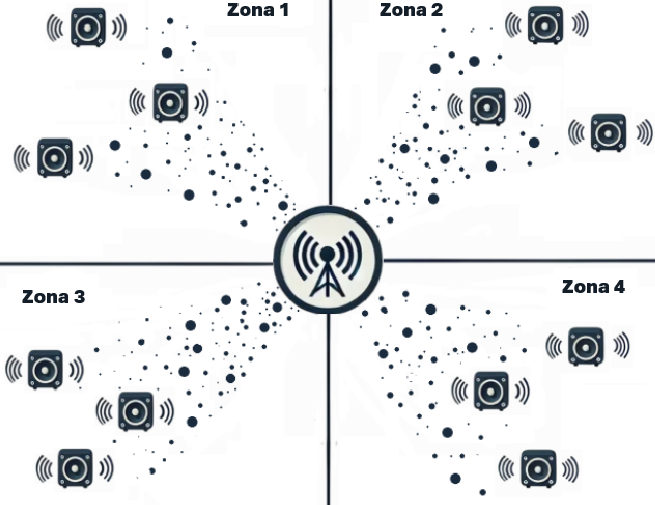
\includegraphics[width=0.6\textwidth]{Screenshot 2024-11-23 164243.png} 
    \caption{Sistema de difusão de áudio digital multi-zona sem fios} % Legenda da imagem
    \label{fig:arquitetura} % Rótulo para referenciar a imagem no texto
\end{figure}


\vspace{2cm}



\subsection{Motivação}

\vspace{0.1cm}


Atualmente, a maioria dos sistemas comerciais de distribuição de áudio baseia-se em infraestruturas cabladas, que, apesar da sua fiabilidade, apresentam limitações significativas em termos de flexibilidade, escalabilidade e custos de instalação, sendo esse os seus maiores defeitos.


Soluções sem fios, por outro lado, são menos comuns e, quando disponíveis, tendem a ser mais restritas a aplicações específicas, como streaming doméstico de música ou transmissões em larga escala, como em estações de rádio. 
Esta realidade evidencia uma lacuna no mercado para um sistema que corresponda a um intermédio aos dois referidos anteriormente, isto é, não existe neste momento um sistema que faça uma distribuição de áudio sem fios multi-canal que seja simultaneamente versátil, com qualidade e aplicável a diferentes contextos, desde pequenos estabelecimentos comerciais até grandes espaços como hotéis, centros comerciais e infraestruturas empresariais.


Assim, o projeto proposto visa preencher este espaço em branco e esta necessidade através do desenvolvimento de um sistema de áudio digital sem fios que promete flexibilidade e personalização. A solução será composta por uma unidade de controlo central e recetores distribuídos, permitindo uma rede de colunas totalmente sincronizada. A arquitetura do sistema permitirá a personalização dinâmica dos canais de áudio em tempo real, ajustando a distribuição do som conforme as necessidades específicas de cada ambiente.
Além da qualidade sonora e da capacidade de adaptação, o sistema destaca-se pela facilidade de instalação e configuração, eliminando a necessidade de infraestruturas complexas e reduzindo custos operacionais e de manutenção. Com um modelo de controlo centralizado e gestão remota intuitiva, esta solução posiciona-se como uma alternativa inovadora e eficiente face a sistemas convencionais tanto públicos como privados.



\vspace{0.8cm}

\subsection{Objetivos}

\vspace{0.3cm}

\begin{enumerate}
\item \textbf{Desenhar a Unidade de Controlo Central:}
\begin{adjustwidth}{0.1cm}{0.1cm}
Este projeto envolve o desenvolvimento de uma unidade central capaz de misturar e distribuir diversas entradas de áudio, como microfone, ficheiro de áudio e streaming, para canais e zonas específicos. Para garantir maior qualidade de som, a unidade contará com funcionalidades de processamento de áudio, incluindo equalização e compressão. Além disso, será desenvolvida uma interface de utilizador intuitiva, projetada para facilitar a gestão e configuração do sistema, permitindo que os utilizadores ajustem e controlem facilmente o áudio de acordo com suas necessidades específicas dos espaços.
\end{adjustwidth}

    

\vspace{0.2cm}

\item \textbf{Adicionar Capacidades Sem Fios:}

\begin{adjustwidth}{0.1cm}{0.1cm}
O objetivo de expandir as capacidades sem fios do sistema envolve integrar a unidade de controlo central a um sistema de difusão sem fios, estabelecendo uma comunicação direta e eficiente entre ambos. É essencial garantir a fiabilidade e a qualidade da transmissão digital, o que será alcançado através de técnicas como buffering e o uso de codecs de áudio. Além disso, o sistema permitirá uma distribuição de áudio adaptativa e sincronizada em todas as saídas de áudio dentro da mesma zona, possibilitando uma experiência auditiva consistente e de qualidade.
\end{adjustwidth}

\vspace{0.2cm}

\item \textbf{Desenhar o Recetor:}

\begin{adjustwidth}{0.1cm}{0.1cm}
O projeto inclui um dispositivo que atuará como intermediário entre a unidade de controle central e as colunas. Esse dispositivo será responsável por receber sinais de áudio transmitidos, selecionar os relevantes e converter esses sinais em sinal elétrico apropriado para ser emitido pela coluna de som.
\end{adjustwidth}

\vspace{0.2cm}

\item \textbf{Desenvolver o Protocolo de Comunicação:}

\begin{adjustwidth}{0.1cm}{0.1cm}
O projeto visa desenvolver um sistema de difusão de áudio digital sem fios que seja versátil, fiável e adaptável a diversos ambientes, desde pequenas lojas até grandes espaços públicos como hotéis, centros comerciais, estádios e feiras ao ar livre. Este sistema pretende aproveitar as vantagens das tecnologias sem fios para oferecer flexibilidade e facilidade de instalação, tornando-o ideal para uso em locais que requerem uma solução de áudio eficaz sem as complicações de uma instalação com fios
\end{adjustwidth}

\end{enumerate}

\newpage

\subsection{Organização do Documento}

\vspace{0.5cm}

Este documento está estruturado em várias secções que abrangem desde o contexto aos progressos realizados. 

\begin{enumerate}
\item \textbf{Trabalhos Relacionados:}
\begin{adjustwidth}{0.1cm}{0.1cm}
Introdução a referências que serviram como inspiração para o projeto, através de estudos prévios no campo da difusão de áudio digital multi-canal sem fios tendo sido realizada uma exploração de sistemas comerciais.
\end{adjustwidth}

    

\vspace{0.2cm}

\item \textbf{Ferramentas e Tecnologias}

\begin{adjustwidth}{0.1cm}{0.1cm}
Explicação detalhada sobre as ferramentas e tecnologias utilizadas no desenvolvimento do sistema, explicando as razões por trás das escolhas feitas. Esta secção abrange os componentes principais, como o nó central, os módulos de comunicação sem fios, os dispositivos recetores e a interface de controlo remoto.

\end{adjustwidth}

\vspace{0.2cm}

\item \textbf{Levantamento de Requisitos e Arquitetura}

\begin{adjustwidth}{0.1cm}{0.1cm}
   Descrição dos requisitos funcionais e não funcionais do sistema e apresentação da arquitetura pensada.
\end{adjustwidth}

\vspace{0.2cm}

\item \textbf{Resultados Esperados}

\begin{adjustwidth}{0.1cm}{0.1cm}
Apresentação dos objetivos principais do sistema e as vantagens esperadas após a sua implementação. Esta secção enfatiza a qualidade do áudio, a eficiência do sistema e o impacto potencial no mercado.
\end{adjustwidth}
\vspace{0.2cm}


\item \textbf{Progressos}

\begin{adjustwidth}{0.1cm}{0.1cm}
   É dada uma visão geral das etapas concluídas e das metas atingidas até o momento, sendo ainda destacado os desafios enfrentados e as soluções implementadas. Esta secção documenta a evolução do projeto nas últimas semanas.
\end{adjustwidth}

\vspace{0.5cm}

\end{enumerate}
Cada secção é projetada para fornecer uma visão abrangente do projeto, desde o seu estado inicial até a sua execução e análise. Ao longo do documento, são relacionadas informações teóricas e práticas para oferecer uma base sólida para a compreensão do trabalho desenvolvido.


\newpage

\section{Trabalhos Relacionados, Ferramentas e Tecnologias}
\hspace{0.5cm}

\subsection{Trabalhos Relacionados}

\vspace{0.1cm}


A evolução dos sistemas de difusão de áudio tem sido impulsionada por avanços tecnológicos que visam melhorar a qualidade sonora, a flexibilidade de instalação e a eficiência da transmissão. Desde os primeiros sistemas analógicos até as atuais soluções digitais e inteligentes, o setor tem sofrido por uma transformação significativa e atualmente, coexistem soluções cabladas e sem fios, tendo cada uma delas vantagens e limitações, dependendo do contexto de aplicação.


Os sistemas cablados, como os oferecidos pela Bosch e Yamaha, são amplamente utilizados em ambientes onde a fiabilidade e a qualidade do sinal são cruciais, como em instalações empresariais, auditórios e infraestruturas de grande escala. Estes são sistemas que garantem uma transmissão estável, minimizando as interferências e permitindo ainda um maior controlo sobre o processamento de áudio. Para além disso, são utilizados protocolos como o Dante e AES67, que permitem a distribuição de áudio sobre redes IP com baixa latência e alta qualidade. No entanto, a sua instalação e manutenção podem ser complexas e dispendiosas, exigindo um planeamento detalhado da infraestrutura. No entanto, a sua instalação e manutenção podem ser complexas e dispendiosas, exigindo um planeamento detalhado da infraestrutura.


Aprofundando brevemente os conceitos citados, o protocolo Dante (Digital Audio Network Through Ethernet) consiste em uma tecnologia desenvolvida pela Audinate para transmissão de áudio digital em redes IP. Este permite a comunicação de múltiplos dispositivos de áudio através de uma rede padrão Ethernet, o que elimina a necessidade de ligações analógicas e acaba por reduzir a complexidade da instalação. Este é amplamente adotado em aplicações profissionais, pois oferece baixa latência, alta qualidade de som e suporte para centenas de canais simultaneamente. Além disso, conta com funcionalidades avançadas de roteamento e gestão remota de dispositivos, o que o torna uma solução eficiente para grandes infraestruturas de áudio. O AES67, por sua vez, é um padrão aberto que visa garantir a integração entre diversos protocolos de áudio sobre IP, tais como Dante, Ravenna e Livewire. Desenvolvido pela Audio Engineering Society (AES), este protocolo define diretrizes comuns para a transmissão de áudio digital, permitindo que sistemas de diferentes fabricantes comuniquem-se de forma integrada. O AES67 é particularmente útil em ambientes onde há necessidade de compatibilidade entre diversas tecnologias, como em estúdios de radiodifusão e instalações de sonorização distribuída. A sua flexibilidade e compatibilidade tornam-no uma escolha popular para projetos que exigem integração de sistemas de áudio diversos.

Por outro lado, empresas como a Sonos e a Bose têm apostado em soluções sem fios, que proporcionam maior flexibilidade e facilidade de instalação, sendo ideais para ambientes domésticos e comerciais de menor dimensão. A Sonos desenvolveu um ecossistema de colunas inteligentes interligadas via Wi-Fi, permitindo a transmissão sincronizada de áudio entre múltiplos dispositivos e possibilitando a configuração personalizada de zonas sonoras. Essa abordagem elimina a necessidade da utilização de cablagem extensa e oferece ainda um controlo intuitivo através de aplicações móveis.

A Tabela~\ref{tab:comparacao_marcas} apresenta uma comparação entre algumas marcas e suas soluções de transmissão de áudio.

\begin{table}[h]
    \centering
    \begin{tabular}{@{}l p{3cm} p{3cm} p{3cm}@{}}
 
        \toprule
        \textbf{Marca} & \textbf{Tecnologia} & \textbf{Pontos Fortes} & \textbf{Pontos Fracos} \\
        \midrule
        Bosch & Cablado (Dante, AES67) & Alta qualidade, estabilidade & Instalação complexa, custo elevado \\
        Yamaha & Cablado (Dante) & Qualidade profissional, baixa latência & Infraestrutura fixa necessária \\
        Sonos & Sem fio (Wi-Fi) & Flexibilidade, fácil instalação & Dependência de conexão Wi-Fi \\
        Bose & Sem fio (Wi-Fi, Bluetooth) & Qualidade premium, usabilidade & Latência maior em relação a sistemas cablados \\
        \bottomrule
    \end{tabular}
    \caption{Comparação entre marcas e suas soluções de transmissão de áudio.}
    \label{tab:comparacao_marcas}
\end{table}




Um exemplo notável deste avanço é a linha de colunas Sonos Era 300 e Era 100, destacada no artigo \textbf{"Com estas colunas da Sonos vai encher a casa de música"}. Estes dispositivos incorporam tecnologias avançadas de espacialização sonora, adaptando-se a diferentes ambientes e proporcionando uma experiência imersiva. Além disso, a capacidade de integração com diversos serviços de streaming e a compatibilidade com padrões de áudio de alta resolução tornam estes sistemas uma referência no mercado de áudio doméstico.
Embora os sistemas sem fios atuais ofereçam uma experiência conveniente e de alta qualidade, a maioria das soluções comerciais permanece focada em aplicações domésticas ou em espaços de menor escala. 


Recentemente, algumas empresas começaram a explorar soluções híbridas, utilizando tecnologias como Bluetooth Low Energy (BLE) e Wi-Fi 6 para melhorar a estabilidade e reduzir a latência da transmissão sem fios. Essas tecnologias permitem reduzir a latência, melhorar a estabilidade do sinal e oferecer uma experiência de áudio mais fluida, especialmente em ambientes onde a conectividade sem fios pode ser um desafio. Algumas das empresas envolvidas nesse estudo são por exemplo a Telit Cinterion, Insight SIP e Silicon Labs que têm investido no desenvolvimento de módulos e sistemas que combinam essas tecnologias para otimizar a transmissão de áudio e comunicação sem fios. 

\newpage

A Tabela~\ref{tab:comparacao_protocolos} apresenta uma comparação entre os protocolos de transmissão de áudio mencionados no texto.

\begin{table}[h]
    \centering
    \begin{tabular}{@{}l p{4cm} p{4cm} p{4cm}@{}}
        \toprule
        \textbf{Protocolo} & \textbf{Tipo} & \textbf{Pontos Fortes} & \textbf{Pontos Fracos} \\
        \midrule
        Dante & Cablado & Alta qualidade, baixa latência, escalabilidade & Requer infraestrutura dedicada, custo elevado \\
        AES67 & Cablado & Padrão aberto, interoperabilidade entre dispositivos & Requer maior largura de banda, mais complexo de configurar \\
        Wi-Fi & Sem fio & Facilidade de instalação, mobilidade & Dependência de rede Wi-Fi, latência maior \\
        Bluetooth & Sem fio & Facilidade de uso, boa compatibilidade com dispositivos pessoais & Alcance limitado, latência maior em relação a sistemas cablados \\
        \bottomrule
    \end{tabular}
    \caption{Comparação entre protocolos de transmissão de áudio mencionados.}
    \label{tab:comparacao_protocolos}
\end{table}



\clearpage
\newpage

\subsection{Descrição do Artigo}
\vspace{0.2cm}

\subsubsection{Modelos e Características Específicas}
\vspace{0.2cm}



\textbf{Era 100:} Este modelo é a evolução das colunas Sonos One, mantendo um design compacto que se adapta facilmente a qualquer ambiente doméstico. A Era 100 oferece conectividade Wi-Fi, permitindo o acesso direto a serviços de streaming sem a necessidade de outros dispositivos intermediários. Esta coluna também incorpora uma interface tátil para controle de volume e reprodução, e suporta a funcionalidade de assistente de voz quando conectada via Wi-Fi, o que amplia suas capacidades de uso sem depender de interações físicas.

\vspace{0.2cm}

\textbf{Era 300:} Destinado a espaços maiores, o Era 300 é conhecido por sua capacidade de emitir "som espacial", criando uma experiência auditiva mais imersiva. Além da conectividade Wi-Fi, este modelo suporta áudio multicanal, permitindo que os usuários desfrutem de som surround sem a necessidade de múltiplas colunas. Assim como a Era 100, ela pode ser controlada via app Sonos, oferecendo uma integração perfeita com o ecossistema de produtos Sonos.
\vspace{1cm}

\subsubsection{Vantagens da Tecnologia Sonos}
\vspace{0.2cm}
\paragraph{Flexibilidade:} As colunas Sonos oferecem uma configuração extremamente flexível, permitindo aos utilizadores conectar várias colunas numa rede Wi-Fi doméstica. Isso possibilita a reprodução sincronizada de música em múltiplos ambientes ou a reprodução de faixas diferentes em cada espaço, tudo controlável através de um aplicativo intuitivo.

\paragraph{Qualidade de Áudio Superior:} Graças à conectividade Wi-Fi, as colunas Sonos são capazes de transmitir áudio de alta resolução, proporcionando uma qualidade sonora significativamente superior à de muitas outras tecnologias sem fio, como o Bluetooth.

\paragraph{Integração com Serviços de Streaming:} As colunas Sonos integram-se perfeitamente com uma vasta gama de serviços de streaming de música, facilitando o acesso a bibliotecas extensas e diversas de conteúdo musical sem a necessidade de hardware adicional.

\newpage
\vspace{1cm}
\subsubsection{Desafios e Limitações da Tecnologia Sonos}
\vspace{0.2cm}
\paragraph{Dependência de uma Conexão Wi-Fi Estável:} Uma das principais limitações das colunas Sonos é a necessidade de uma conexão Wi-Fi constante e estável. Interrupções na rede podem afetar diretamente a reprodução de música, resultando em interrupções ou perda de conectividade.

\paragraph{Alcance Limitado:} O alcance da conectividade Wi-Fi é também uma restrição, especialmente em ambientes maiores ou com múltiplas barreiras físicas, como paredes densas, que podem interferir e limitar a distribuição do sinal.

\vspace{1cm}

\subsubsection{Conclusão e Lições aprendidas}

Ao explorar o sistema de áudio multicanal via Wi-Fi da Sonos, certas lições podem ser valiosas no desenvolvimento do nosso sistema. A integração de várias colunas numa rede doméstica destaca a eficácia da tecnologia Wi-Fi em proporcionar uma experiência auditiva consistente e de qualidade.

A flexibilidade do sistema Sonos em permitir o controlo individual ou sincronizado das colunas em diferentes ambientes ilustra a importância de um design centrado no utilizador. Este aspecto deve ser considerado ao desenvolver um novo sistema, onde o utilizador pode gerir a experiência auditiva dos clientes remotamente, através de um website. A facilidade de uso é essencial para permitir que o proprietário posso iniciar/parar o audio bem como ajustes do volume desejado nas diferentes zonas, oferecendo um ambiente sonoro que pode ser modificado dinamicamente para atender às preferências dos clientes ou ao tema do evento que irá ocorrer.

A capacidade de manter a qualidade do som através da rede Wi-Fi ressalta a necessidade de escolher tecnologias de transmissão adequadas que suportem a fiabilidade de áudio desejada.

Com o que aprendemos com estas lições, é possível desenvolver um sistema de áudio multicanal via Wi-Fi que não só atenda às expectativas modernas de funcionalidade e desempenho, mas que também proporcione uma experiência auditiva envolvente e adaptável.

\newpage

\subsection{Ferramentas e Tecnologias}


O projeto propõe uma solução versátil para a transmissão de áudio multicanal. Para isso, diversas tecnologias foram estudadas e selecionadas com base em critérios como estabilidade, custo-benefício e facilidade de implementação.

\subsubsection{Comunicação via Wi-Fi}
A comunicação entre os dispositivos será realizada exclusivamente via Wi-Fi, aproveitando sua ampla disponibilidade, facilidade de configuração e suporte a redes sem fio de alta velocidade. Sempre que possível, serão utilizadas redes Wi-Fi dedicadas para evitar congestionamentos e garantir maior estabilidade na transmissão de áudio. Essa abordagem irá reduzir a necessidade de usar cabos, o que facilita a instalação e manutenção e aumenta também a flexibilidade do sistema.

A escolha do Wi-Fi como tecnologia de comunicação foi feita com base nas suas vantagens a nível de flexibilidade, facilidade de instalação e custo-benefício, em comparação com outras opções, como Ethernet e Power Line Communication (PLC).

A Tabela~\ref{tab:tecnologias_comparacao} ilustra as principais vantagens e desvantagens de diferentes tecnologias de transmissão.

\begin{table}[h]
    \centering
    \begin{tabular}{@{}l p{10cm}@{}}
        \toprule
        \textbf{Tecnologia} & \textbf{Vantagens e Desvantagens} \\
        \midrule
        Ethernet & Proporciona uma conexão estável e de baixa latência, sendo ideal para aplicações que exigem alta confiabilidade e largura de banda consistente. No entanto, requer infraestruturas de cabeamento, o que pode aumentar a complexidade da instalação e os custos associados, especialmente em ambientes onde a mobilidade é um fator importante. \\
        Wi-Fi & Oferece grande flexibilidade e facilidade de configuração, sendo amplamente utilizado devido à sua acessibilidade e capacidade de suporte a múltiplos dispositivos. No entanto, sua performance pode ser impactada por interferências e congestionamentos, especialmente em redes não dedicadas. \\
        PLC (Power Line Communication) & Utiliza a infraestrutura elétrica existente para a transmissão de dados, eliminando a necessidade de novos cabeamentos. Apesar de ser uma solução prática para ambientes onde a instalação de redes cabeadas não é viável, pode apresentar limitações de alcance e estar sujeita a interferências provenientes de variações na rede elétrica. \\
        RF (Rádio Frequência) & Alternativa sem fio que oferece grande alcance, tornando-se viável para transmissões em locais amplos ou remotos. No entanto, está sujeita a interferências de outros dispositivos operando na mesma faixa de frequência e pode exigir conformidade com regulamentações específicas para evitar conflitos de espectro. \\
        \bottomrule
    \end{tabular}
    \caption{Comparação entre diferentes tecnologias de transmissão.}
    \label{tab:tecnologias_comparacao}
\end{table}


\subsubsection{Protocolos de Transmissão de Dados}
A transmissão de áudio será baseada no protocolo multicast, que otimiza a utilização da largura de banda ao enviar dados apenas para dispositivos que optaram por recebê-los. O protocolo multicast permite que uma única fonte envie pacotes de dados para múltiplos receptores simultaneamente, sem a necessidade de duplicar a transmissão para cada um deles. Dessa forma, a rede não é sobrecarregada com tráfego redundante, melhorando a eficiência e reduzindo o consumo de recursos. Isso reduz significativamente o tráfego desnecessário e melhora a eficiência da rede, sendo ideal para sistemas de áudio e vídeo que requerem transmissão para múltiplos receptores simultaneamente.

Alternativamente, pode-se considerar o uso do broadcast, que transmite dados para todos os dispositivos na rede. Diferente do multicast, o broadcast envia pacotes para todos os nós da rede, independentemente de eles terem interesse na informação. Isso pode gerar tráfego desnecessário, aumentando a latência e sobrecarregando a infraestrutura da rede, especialmente em grandes ambientes. A escolha entre multicast e broadcast dependerá dos testes e requisitos específicos do sistema. A Tabela~\ref{tab:comparacao_multicast_broadcast} apresenta uma comparação detalhada entre essas abordagens.

\begin{table}[h]
    \centering
    \begin{tabular}{@{}l p{5cm} p{5cm}@{}}
        \toprule
        \textbf{Protocolo} & \textbf{Implementação} & \textbf{Desvantagens} \\
        \midrule
        Broadcast & Emissão para todos os dispositivos da rede & Maior tráfego desnecessário, podendo impactar o desempenho da rede \\
        Multicast & Emissão para dispositivos pré-definidos & Requer configuração nos grupos de recepção, pode exigir suporte da infraestrutura de rede \\
        \bottomrule
    \end{tabular}
    \caption{Comparação entre Broadcast e Multicast.}
    \label{tab:comparacao_multicast_broadcast}
\end{table}


\subsubsection{Arquitetura do Sistema} O sistema será controlado por um nó central operando em um Raspberry Pi, devido à sua robustez, relação custo-benefício e suporte a uma ampla variedade de protocolos de comunicação. Este dispositivo será responsável por gerir a transmissão de áudio, coordenar os recetores e disponibilizar uma interface de controlo remoto através de um Website. Essa interface permitirá que os usuários ajustem configurações de áudio de forma intuitiva, utilizando qualquer dispositivo conectado à rede.

Os recetores do sistema também serão baseados em Raspberry Pi's, mas poderá ser considerada uma abordagem alternativa com dispositivos de menor custo, dependendo dos requisitos finais do projeto. Essa abordagem permite maior escalabilidade, suporte a redes IP e reprodução de áudio com qualidade satisfatória. A conexão entre o nó central e os recetores será feita via Wi-Fi, garantindo mobilidade e simplificação na instalação.


\subsubsection{Protocolos de Streaming de \'Audio}
Al\'em das tecnologias de comunica\c{c}\~ao, a escolha dos protocolos de streaming de \'audio \'e essencial para garantir uma transmiss\~ao eficiente e em tempo real entre a unidade central e os recetores. Foram analisados alguns protocolos, incluindo RTSP, Icecast, WebRTC e MQTT Audio.

\begin{itemize}
    \item \textbf{RTSP (Real-Time Streaming Protocol)}: Amplamente utilizado para o controle de fluxos de m\'idia em tempo real, permitindo comandos como play, pause e stop. Ele \'e frequentemente combinado com o RTP (Real-Time Transport Protocol) para a transmiss\~ao dos pacotes de \'audio, garantindo baixa lat\^encia e sincroniza\c{c}\~ao precisa. Esse protocolo \'e ideal para aplica\c{c}\~oes interativas, onde o usu\'ario pode iniciar ou interromper a transmiss\~ao sob demanda.
    \item \textbf{Icecast}: Solu\c{c}\~ao de c\'odigo aberto para streaming cont\'inuo de \'audio, muito utilizada em r\'adios online. Suporta diversos formatos e oferece uma configura\c{c}\~ao flex\'ivel, sendo adequado para redes locais e sistemas personalizados, como o proposto neste projeto. Sua simplicidade e efici\^encia o tornam uma alternativa vi\'avel para transmiss\~oes de \'audio em tempo real, especialmente em sistemas onde o foco \'e a distribui\c{c}\~ao cont\'inua do conte\'udo sem necessidade de controle interativo.
    \item \textbf{WebRTC (Web Real-Time Communication)}: Protocolo projetado para comunica\c{c}\~ao em tempo real diretamente entre navegadores e dispositivos, sem a necessidade de servidores intermedi\'arios. Possui suporte nativo para baixa lat\^encia e transmiss\~ao de m\'idia bidirecional, tornando-o ideal para aplica\c{c}\~oes interativas que envolvem comunica\c{c}\~ao direta entre usu\'arios.
    \item \textbf{MQTT Audio}: Embora originalmente projetado para a comunica\c{c}\~ao eficiente entre dispositivos IoT, o MQTT tamb\'em pode ser usado para transmiss\~ao de \'audio em redes locais. Sua abordagem baseada em publica\c{c}\~ao/assinatura permite um gerenciamento eficiente do tr\'afego, sendo uma op\c{c}\~ao interessante para sistemas distribu\'idos onde a otimiza\c{c}\~ao da largura de banda \'e essencial.
\end{itemize}

\begin{table}[h]
    \centering
    \begin{tabular}{@{}l p{5cm} p{5cm}@{}}
        \toprule
        \textbf{Protocolo} & \textbf{Vantagens} & \textbf{Desvantagens} \\
        \midrule
        RTSP & Baixa lat\^encia e controle interativo & Requer infraestrutura de servidor \\
        Icecast & Suporte a diversos formatos e simples de configurar & Maior lat\^encia em compara\c{c}\~ao com RTSP e WebRTC \\
        WebRTC & Baixa lat\^encia e comunica\c{c}\~ao P2P & Pode ser complexo de implementar \\
        MQTT Audio & Efici\^encia em redes distribu\'idas & N\~ao foi projetado originalmente para transmiss\~ao de \'audio \\
        \bottomrule
    \end{tabular}
    \caption{Compara\c{c}\~ao entre diferentes protocolos de streaming de \'audio.}
    \label{tab:comparacao_protocolos_audio}
\end{table}

Estes protocolos revelam características pertinentes e podem ser adaptados à arquitetura do sistema, garantindo um streaming confiável, com baixa latência e suporte a múltiplos formatos de áudio.

\subsubsection{Conclusão} A escolha das ferramentas e tecnologias para este projeto foi guiada por critérios como eficiência, flexibilidade, custo-benefício e facilidade de implementação. A utilização de Wi-Fi como meio de comunicação garante uma instalação simplificada e acessível, enquanto o uso de protocolos adequados para transmissão de áudio assegura qualidade e baixa latência. O sistema centralizado baseado em Raspberry Pi proporciona uma solução robusta e escalável, permitindo ajustes conforme as necessidades do utilizador.
Através da combinação dessas tecnologias modernas e acessíveis, o projeto visa oferecer uma solução eficiente para a transmissão de áudio multicanal, adequada para ambientes audiovisuais, com foco na estabilidade, integração simplificada e flexibilidade operacional.





\newpage


\section{Cenário, Levantamento de requisitos e Arquitetura}

\subsection{Cenário}


\textbf{Hotel} (Comunica\c{c}\~ao via Wi-Fi)

Clara, gerente de um hotel, está organizando o ambiente de áudio para diferentes zonas do hotel durante uma tarde movimentada. O sistema de difusão de áudio permite uma gestão eficiente e centralizada, garantindo que cada área do hotel tenha um ambiente sonoro adequado às suas necessidades específicas.

No hotel, existem diferentes tipos de zonas com requisitos sonoros distintos. Na recepção e lobby, é essencial uma música ambiente suave e relaxante para proporcionar uma experiência acolhedora aos hóspedes que estão chegando ou aguardando atendimento. No restaurante, um fundo musical discreto ajuda a criar uma atmosfera confortável sem interferir na comunicação entre os clientes. Já nas salas de conferências e eventos, a necessidade é diferente: o sistema deve permitir transmissões de áudio direcionadas, garantindo que palestras e apresentações sejam ouvidas com clareza.

Na área da piscina e do jardim, onde o ambiente é mais descontraído, Clara utiliza uma playlist animada e leve, adaptada à dinâmica desses espaços. Todas as zonas são conectadas ao sistema de transmissão digital por meio de uma rede Wi-Fi dedicada, garantindo qualidade de áudio sem interrupções em qualquer ambiente.

Clara interage com o sistema através de uma interface web a partir do seu PC ou de um dispositivo móvel. O painel de controlo permite-lhe ajustar, em tempo real, o volume em cada zona e alternar entre diferentes playlists conforme necessário. Por exemplo, ao notar um aumento de movimento na piscina, ela pode rapidamente alterar para uma playlist mais vibrante e apropriada para o espaço, garantindo que a experiência dos hóspedes seja sempre personalizada e ajustada ao ambiente.

Com a solução de Wi-Fi, Clara garante a flexibilidade e o controlo total sobre a transmissão de áudio, assegurando que cada área do hotel recebe o som adequado sem comprometer a experiência dos hóspedes. O sistema ainda permite automações programáveis, como playlists específicas para diferentes horas do dia ou dias da semana, garantindo uma gestão sonora eficiente e sem necessidade de supervisão constante.

\newpage 

\textbf{Outros Cenários de Aplicação}

Embora este sistema seja particularmente vantajoso para o setor hoteleiro, sua aplicação pode ser estendida a outros cenários, como:

\begin{itemize}
    \item \textbf{Centro Comercial: } Em grandes centros comerciais, cada loja pode necessitar de um canal de áudio independente para oferecer uma experiência personalizada aos clientes. Algumas áreas podem ter música ambiente relaxante, enquanto outras podem precisar de transmissões promocionais ou informações de serviço.

    \item  \textbf{Universidades e Instituições de Ensino:} Em ambientes educacionais, salas de aula podem receber áudios diferenciados conforme as necessidades dos professores, incluindo transmissões de aulas remotas ou mensagens institucionais.

    \item \textbf{Escritórios e Espaços Corporativos: } Empresas podem usar este sistema para criar um ambiente produtivo, gerindo a distribuição de música ambiente em escritórios abertos ou fornecendo mensagens direcionadas para diferentes departamentos.
    
\end{itemize}


\hspace{5cm}


\textbf{Desafios Encontrados}

Apesar das vantagens da transmissão sem fios, alguns desafios foram encontrados após a definição destes cenários. Um dos principais é manter a estabilidade da rede Wi-Fi, especialmente em locais onde há grande movimentação de pessoas e dispositivos conectados. Num hotel, por exemplo, o tráfego de rede pode aumentar significativamente em momentos específicos, como no horário do pequeno-almoço, quando muitos hóspedes utilizam seus dispositivos móveis.

Além disso, a latência e sincronização do áudio são fatores essenciais para uma experiência auditiva imersiva. No caso do shopping center, onde múltiplas zonas podem estar transmitindo conteúdos diferentes ao mesmo tempo, o sistema deve garantir que os áudios estejam perfeitamente sincronizados, evitando atrasos perceptíveis entre os ambientes.





\newpage


\hspace{5cm}
\subsection{Levantamento de Requisitos e Arquitetura} 

\hspace{2cm}

Com base no cenário apresentado, foi realizado um levantamento de requisitos. Para permitir a gestão do sistema de som por parte de um cliente, será disponibilizado um website, acessível através do PC do cliente, onde o responsável poderá ajustar a música para as zonas desejadas de forma intuitiva. Após a seleção do áudio no website, a informação é transmitida ao Nó Central, que desempenha um papel fundamental na arquitetura do sistema. 


\hspace{0.5cm}

O Nó Central é responsável por realizar a gestão global dos fluxos de áudio e coordenar a sua distribuição para os recetores nas respetivas zonas. Ele opera como o ponto de integração central do sistema, garantindo que os sinais de áudio são processados, organizados e enviados corretamente para os destinos apropriados.



Este recebe dados de áudio provenientes de várias fontes, incluindo o microfone ou arquivos armazenados localmente no sistema. Ele processa os sinais, adaptando o formato. Para além disso, o Nó Central garante que cada zona receba o conteúdo correto. No Nó Central são armazenados arquivos de áudio e informações essenciais numa base de dados local.


\hspace{0.5cm}

Posto isto, a audio atribuido à respetiva zona é enviado para o router que será o responsável
por estabelecer a comunicação sem fios entre o nó central e os dispositivos recetores. Ele recebe os sinais de áudio do nó central e transmite-os para os diferentes recetores e consequentemente para as respetivas colunas, que estão distribuídos nas diversas zonas. 



\hspace{5cm}



Na arquitetura apresentada abaixo, é possível ver uma representação do esquema correspondente a uma única zona do sistema estando esta seguida de uma representação do nó central de forma mais detalhada. Esta configuração pode ser replicada para as diversas zonas. Essa escalabilidade permite que o sistema seja facilmente adaptado para aplicações com múltiplas zonas de áudio.


Na arquitetura apresentada abaixo, é possível observar uma representação de uma única zona do sistema, seguida por uma representação mais detalhada do nó central. Essa configuração pode ser replicada para outras zonas, proporcionando escalabilidade ao sistema, o que permite sua adaptação para aplicações com múltiplas zonas de áudio.


\hspace{2cm}


\begin{figure}[h!] % Ambiente para inserir a imagem
    \centering % Centraliza a imagem
    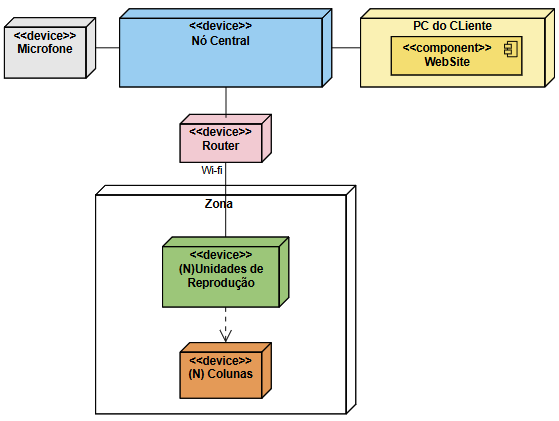
\includegraphics[width=0.75\textwidth]{Screenshot 2024-12-07 171502.png} 
    \caption{Diagrama de Arquitetura do Sistema} % Legenda da imagem
    \label{fig:arquitetura} % Rótulo para referenciar a imagem no texto
\end{figure}



\hspace{2cm}


\begin{figure}[h!] % Ambiente para inserir a imagem
    \centering % Centraliza a imagem
    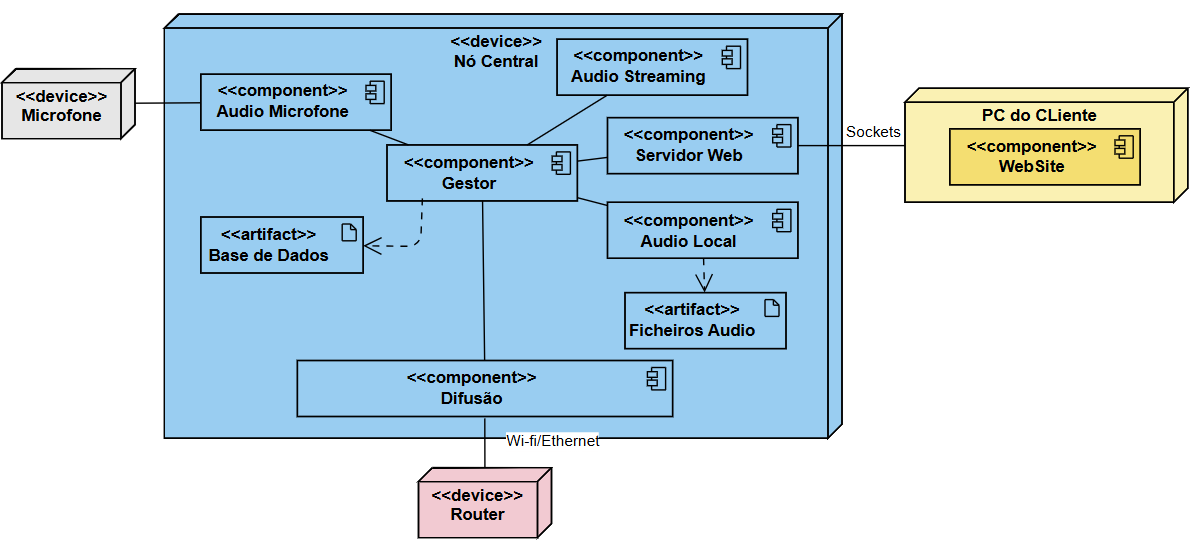
\includegraphics[width=0.90\textwidth]{arq1.png} 
    \caption{Nó Central} % Legenda da imagem
    \label{fig:arquitetura} % Rótulo para referenciar a imagem no texto
\end{figure}

\clearpage
\newpage



\section{Progressos}


O desenvolvimento do projeto foi estruturado em etapas sequenciais, começando pela utilização de Wi-Fi, escolhido pela sua simplicidade de implementação. Para a demonstração, estabelecemos como objetivo a criação de três canais de áudio distintos: streaming de voz, reprodução de ficheiros de áudio e transmissão em tempo real.

O trabalho inicial focou-se na extração e reprodução das três fontes de áudio no mesmo computador. Esta etapa revelou-se mais demorada, especialmente no caso do streaming de voz e da transmissão em tempo real, devido à sua maior complexidade. Apesar disso, conseguimos concluir esta fase com sucesso.

Posteriormente, avançámos para a transmissão de áudio para um segundo computador, utilizando o protocolo UDP, que também foi implementada com êxito.

Atualmente, estamos a trabalhar no desenvolvimento do UDP broadcast, que permitirá a transmissão simultânea para múltiplos dispositivos. No entanto, esta fase está a enfrentar alguns desafios técnicos, o que tem causado atrasos no progresso planeado.

\clearpage
\newpage


\section{Resultados Esperados}

O desenvolvimento do sistema de difusão de áudio digital multi-canal tem como objetivo proporcionar uma experiência sonora com clareza e precisão em todas as zonas cobertas. A utilização de tecnologias sem fios permite uma cobertura extensa e flexível, eliminando a necessidade de infraestrutura física complexa e facilitando ajustes ou expansões conforme as necessidades do ambiente. Espera-se que a unidade de controlo central ofereça funcionalidades avançadas de gestão remota, permitindo a personalização dinâmica dos canais de áudio para atender às exigências específicas de diferentes cenários.

\hspace{2cm}

\subsection{Qualidade e Experiência do Usuário}
Um dos principais focos do sistema é a \textbf{qualidade do áudio}, garantindo que a transmissão seja clara, sem ruídos ou interferências. Para isso, serão implementadas tecnologias de \textbf{compressão eficiente de áudio} e protocolos de transmissão de \textbf{baixa latência}, assegurando que não haja atrasos perceptíveis na distribuição do som, mesmo entre múltiplas zonas.

Outro aspecto fundamental é a \textbf{sincronização precisa} entre as zonas, evitando descompassos e garantindo que o áudio reproduzido em diferentes áreas permaneça harmonioso. Além disso, espera-se que o sistema ofereça \textbf{opções de equalização personalizadas}, permitindo ajustes específicos para cada ambiente (por exemplo, reforço de graves em áreas de entretenimento e som mais suave em zonas de relaxamento).

A \textbf{interface de usuário} será projetada para ser intuitiva e acessível, garantindo que tanto operadores experientes quanto usuários comuns possam controlar o sistema de forma eficiente. A gestão do áudio poderá ser feita via um website responsivo, compatível com dispositivos móveis, proporcionando flexibilidade e facilidade de uso.

\hspace{2cm}

\subsection{Benefícios Operacionais e Redução de Custos}
A abordagem sem fios do sistema reduz significativamente os custos operacionais em comparação com soluções tradicionais cabladas. A instalação será mais rápida e menos intrusiva, minimizando a necessidade de infraestrutura adicional e permitindo maior flexibilidade na disposição das colunas de som.

\hspace{2cm}
\newpage

\subsection{Desafios Encontrados}


\subsection{Conclusão}
Após a implementação e os períodos de teste, espera-se que o sistema supere as expectativas em termos de qualidade sonora, usabilidade e confiabilidade. O projeto tem potencial para contribuir significativamente para o avanço do conhecimento e da tecnologia no campo da engenharia de áudio e telecomunicações, fornecendo dados valiosos para futuras investigações e aplicações práticas na área. Além disso, sua flexibilidade e capacidade de adaptação a diferentes contextos garantem que ele possa ser utilizado em diversos setores, como hotelaria, comércio, eventos e ambientes corporativos. Com a implementação bem-sucedida, o sistema poderá servir como referência para futuras inovações em sistemas de difusão de áudio digital.


\newpage


\section*{Webgrafia}

\begin{itemize}
    \item \textbf{Bosch Security.} (s.d.). \textit{Soluções de áudio comercial para endereços públicos}. Acedido em 27 de novembro de 2024, de \url{https://www.boschsecurity.com/xl/pt/solucoes/solucoes-para-enderecos-publicos/sistemas-de-audio-comercial/}
    
    \item \textbf{K2Ponto.} (s.d.). \textit{O que é o protocolo RTSP e para que ele serve?}. Acedido em 27 de novembro de 2024, de \url{https://k2ponto.com.br/blog/o-que-e-o-protocolo-rtsp-e-para-que-ele-serve/}
    
    \item \textbf{NetSecCloud.} (s.d.). \textit{Understanding Multicast and Broadcast: A Beginner’s Guide}. Acedido em 27 de novembro de 2024, de \url{https://netseccloud.com/understanding-multicast-and-broadcast-a-beginner-s-guide}
    
    \item \textbf{Sonos.} (s.d.). \textit{Com estas colunas da Sonos vai encher a casa de música}. Acedido em 27 de novembro de 2024, de \url{https://www.must.jornaldenegocios.pt/viver/detalhe/com-estas-colunas-da-sonos-vai-encher-a-casa-de-musica}
    
    \item \textbf{Wikipedia.} (s.d.). \textit{Icecast}. Acedido em 27 de novembro de 2024, de \url{https://en.wikipedia.org/wiki/Icecast}
    
    \item \textbf{Wikipedia.} (s.d.). \textit{PLC}. Acedido em 27 de novembro de 2024, de \url{https://pt.wikipedia.org/wiki/PLC}
    
    \item \textbf{Wikipedia.} (s.d.). \textit{RTSP}. Acedido em 27 de novembro de 2024, de \url{https://pt.wikipedia.org/wiki/RTSP}
\end{itemize}



\end{document}